\chapter{Descripcción del metodo}

En este capítulo se describe el método de seguimiento seleccionado para este trabajo.
Primero, en la Sección \ref{sec:ac} se explica el algoritmo utilizado \emph{Contornos Activos},
y en la Sección \ref{sec:impl} su implementación. Luego, en la Sección \ref{sec:eleccion}
se justifica la elección del algoritmo. Finalmente, en la Sección \ref{sec:ac-problemas}
se analiza las limitaciones del algoritmo para esta aplicación.


\section{Contornos Activos}
\label{sec:ac}

La segmentación basada en contornos activos se basa en definir una región en base a su contorno.
El contorno o borde de una región $\Omega_i$ se representa por una curva paramétrica dada por:

\begin{equation}
    C_i(s) = (x_i(s), y_i(s))
\end{equation}

donde $0 \leq s \leq S_i$, y $C_i(0) = C_i(S_i)$, siendo $S_i$ el total de puntos que conforman la curva.
Es decir, $C_i$ es una curva cerrada.

Se definen tantos contornos como objetos de interés haya en la secuencia ($i$ es un entero entre 1 y el número de objetos).
Adicionalmente, se considera una región $\Omega_0$ que contiene a todo punto que no forma parte de ninguna otra región.
Se la denomina \textit{región de fondo}.

Se declara una función de probabilidad $p$ que permite saber que tan probable es que un píxel forme parte de una dada región.
Para esto, es necesaria una función $v$ que dado un píxel, devuelve un vector $v(x)$ de caracteristicas, por ejemplo los valores RGB del pixel.
Esto permite calcular $p(v(x) \vert \Omega_i)$, la probabilidad de que un píxel $x$ forme parte de una región $\Omega_i$ .
Estas funciones dependen de la secuencia particular a ser analizada, por lo que varían dependiendo del caso de estudio.
Como ejemplo, se toman los valores RGB como vector de características y
$p(v(x) \vert \Omega_i) = \| v(x) - v_i \| $, donde $v_i$ es el valor promedio RGB de todo pixel en la región $\Omega_i$.

Se define la función de energía de los contornos:

\begin{equation}
    \label{eq:ac-energy}
    E = - \sum_{m=0}^{M}{\int_{\Omega_m}{\log{p(v(x) \vert \Omega_m)} dx} + \lambda \int_{C_m}{ds}}
\end{equation}

Los algoritmos basados en contornos activos, buscan minimizar esta ecuación. Si el valor de $E$ es mínimo para un cuadro, se
debería haber encontrado la mejor aproximación de la región de los objetos interés. De \ref{eq:ac-energy} se
deriva la ecuación de evolución de cualquier curva $C_m$:

\begin{eqnarray}
    \frac{dC_m}{dt} &=& (F_d + F_s) \overrightarrow{N}_{C_m} \\
    F_d &=& \log{p(v(x) \vert \Omega_m) / p(v(x) \vert \Omega_0)} \\
    F_s &=& \lambda \kappa_m \label{eq:ac-formal}
\end{eqnarray}

$F_d$ y $F_s$ son fuerzas derivadas de la ecuación de energía. $F_d$ representa la competencia entre regiones y $F_s$ un
suavizado. $\kappa_m$ es la curvatura de la curva $C_m$.

Existe otra formulación del problema de evolución de curvas, que consiste en
representar la curva como el nivel cero de una superficie $\phi$ (ver \cite{Osher88}).

\section{Implementación Numérica}
\label{sec:impl}

Se toma de referencia la implementación segun \citeauthor{fast-level-set} (ver \cite{fast-level-set}).
En la implementación, el borde de un contorno $C_m$ se representa usando dos conjuntos de píxeles
correspondientes a los bordes interno y externo, $L_{in}$ y $L_{out}$
respectivamente. Entonces, la evolución se realiza intercambiando píxeles entre
estos dos conjuntos.

A continuación se detalla la técnica para la segmentación de un solo objeto de
interés que se puede fácilmente extrapolar y utilizar para la
segmentación de múltiples objetos
\footnote{Para la segmentación de múltiples objetos basta con marcar las distintas regiones con un identificador
distinto y seguirlas por separado.}.

El objeto de interés $\Omega_{1}$ y el fondo $\Omega_{0}$ cumplen
$\Omega_{1}\cup\Omega_{0} = I_{k}$ donde $I_{k}$ es la imagen del cuadro $k$ de
la secuencia de imágenes, y $\Omega_{1}\cap\Omega_{0} = \emptyset$. Cada una de
las regiones está caracterizada por su vector característico $v_{m}, m =
\{0,1\}$.

Se define una función $\phi(x)$ que indica si un píxel $x$ pertenece a una región o al fondo de la siguiente manera:

\begin{equation}
\phi(x) =
\left\{
    \begin{array}{ll}
        3  & \mbox{si } x \in \Omega_{0} \mbox{  y  } x \notin L_{out} \\
        1  & \mbox{si } x \in L_{out}\\
        -1  & \mbox{si } x \in L_{in}\\
        -3 & \mbox{si } x \in \Omega_{1} \mbox{  y  } x \notin L_{in} \\
    \end{array}
\right.
\end{equation}

Los conjuntos $L_{in}$ y $L_{out}$ se definen como

\begin{equation}
    L_{in} = \{ x \mbox{ es un píxel } \vert \mbox{    }  \phi(x) < 0 \mbox{ y } \exists y \in N_{4}(x) \mbox{ de modo que } \phi(y) > 0 \}
\end{equation}

\begin{equation}
    L_{out} = \{ x \mbox{ es un píxel } \vert \mbox{    } \phi(x) > 0 \mbox{ y } \exists y \in N_{4}(x) \mbox{ de modo que } \phi(y) < 0 \}
\end{equation}

donde $N_{4}(x) = \{ y \mbox{ es un pixel } \vert \mbox{   } |x-y| = 1 \}$, son los píxeles
vecinos del píxel $x$.

El algoritmo de segmentación es un algoritmo de dos ciclos, ya que luego de la
especificación inicial de la curva en forma supervisada \footnote{Podría no ser
supervisada. Existen variantes con determinaciones semi-supervisadas del objeto
de interés, así como también detección automática basada en ciertas
características predefinidas.} se intercambian los píxeles de $L_{in}$ y
$L_{out}$ en dos ciclos. En el primero, se aplica la fuerza $F_{d}(x)$, y en el
segundo se aplica $F_{s}(x)$ para la regularización.

En el primer ciclo, se ejecutan los siguientes pasos $N_{a}$ veces, donde $ 0 <
N_{a} < max(filas, columnas)$.

\begin{enumerate}

    \item Para cada $x \in L_{out}$, si $F_{d}(x) > 0$ entonces borrar $x$ de $L_{out}$ y agregarlo a $L_{in}$. \\
    Luego, $\forall y \in N_{4}(x)$, con $\phi(y) = 3$, agregar $y$ to $L_{out}$ y hacer $\phi(y) = 1$.

    \item Después del paso 1 algunos de los píxeles $x$ en $L_{in}$ pasan a ser píxeles internos. \\
    Por lo tanto, se sacan de $L_{in}$ y se hace $\phi(x) = -3$.

    \item Para cada $x \in L_{in}$ , si $F_{d}(x) < 0$ entonces, borrar $x$ de $L_{in}$ y agregarlo a $L_{out}$. \\
    Luego, $\forall y \in N_{4}(x)$, con $\phi(y) = -3$, agregar $y$ a $L_{in}$ y hacer $\phi(y) = -1$.


    \item Después del paso 3 algunos de los píxeles $x$ en $L_{out}$ pasan a ser píxeles externos. \\
    Por lo tanto, se sacan de $L_{out}$ y se hace $\phi(x) = 3$.

\end{enumerate}

En el segundo ciclo, la curva se suaviza utilizando un filtro Gaussiano, de tal
forma que la fuerza de evolución es $F_{s}(x) = G \otimes \phi(x)$. Para aplicar $F_s$ se usan los mismos
pasos que para $F_d$. El resultado final es análogo a modificar la curva de acuerdo
a la definición formal dada anteriormente (Ecuación \ref{eq:ac-formal}).

En cada cuadro, el borde del contorno del objeto es actualizado de acuerdo al
resultado obtenido por el algoritmo en el cuadro anterior. En el caso de la
primera imagen, se puede dar de forma supervisada o semi-supervisada por el
usuario, o bien puede ser obtenida de forma automática mediante algoritmos de
aprendizaje complejos basados en características predefinidas.

El algoritmo termina cuando se alcanza la condición de corte, dada por las
ecuaciones \ref{eq:active-contours-stoppingCondition} o cuando se alcanza el numero de iteraciones $N_a$

\begin{equation}
\label{eq:active-contours-stoppingCondition}
    \begin{array}{ll}
        F_{d}(x) \leq 0 & \forall x \in L_{out}\\
        F_{d}(x) \leq 0 & \forall x \in L_{in}
    \end{array}
\end{equation}

\section{Elección}
\label{sec:eleccion}

Se elegio el algoritmo \emph{Contornos Activos} por varios motivos:
\begin{itemize}
\item No depende de disponer de bloques de $n x n$ pixeles para su correcto funcionamiento. Una de
las principales restricciones de este trabajo es utilizar una sola camara para obtener el video, y
como se explica en la sección \ref{sub-sec:camaras} un jugador esta formado por un numero muy limitado de pixeles, dificultando el uso de algoritmos que no tengan esta caracteristica.

\item Su tiempo de ejecución no depende del tamaño del cuadro, sino de los jugadores. Esto hace que sea muy rapido de ejecutar por cuadro, posibilitando el análisis en tiempo real.

\item Se cuenta con metodos de manejo de oclusiones para \emph{Contornos Activos}\cite{paper-juliana}.

\end{itemize}

\section{Limitaciones}
\label{sec:ac-problemas}

El correcto funcionamiento del algoritmo de contornos
activos\cite{fast-level-set} depende de una buena selección de la función
característica, para poder distinguir claramente a un jugador respecto a otros
objetos o respecto del fondo. En casos como el ilustrado por la figura
\ref{fig:camiseta}, elegir una función característica resulta sencillo, ya que
con elegir el color de la camiseta se asegura una buena descripción del contorno
a seguir. Sin embargo, la imagen de la figura \ref{fig:camiseta-rayada} introduce
uno de los problemas en la selección de la función característica. Se puede ver que
las diferencias entre ambos colores del objeto hacen dificil identificarlos a ambos
con una misma caracteristica.

\begin{figure}[H]
    \centering
    \begin{minipage}[t]{.5\textwidth}
        \centering
        
\includegraphics[width=.4\linewidth]{./images/rect2995.png}
        \captionof{figure}{Camiseta de color lisa. El color de la camiseta es claramente distinguible del fondo.}
        \label{fig:camiseta}
    \end{minipage}%
    \begin{minipage}[t]{.5\textwidth}
        \centering
        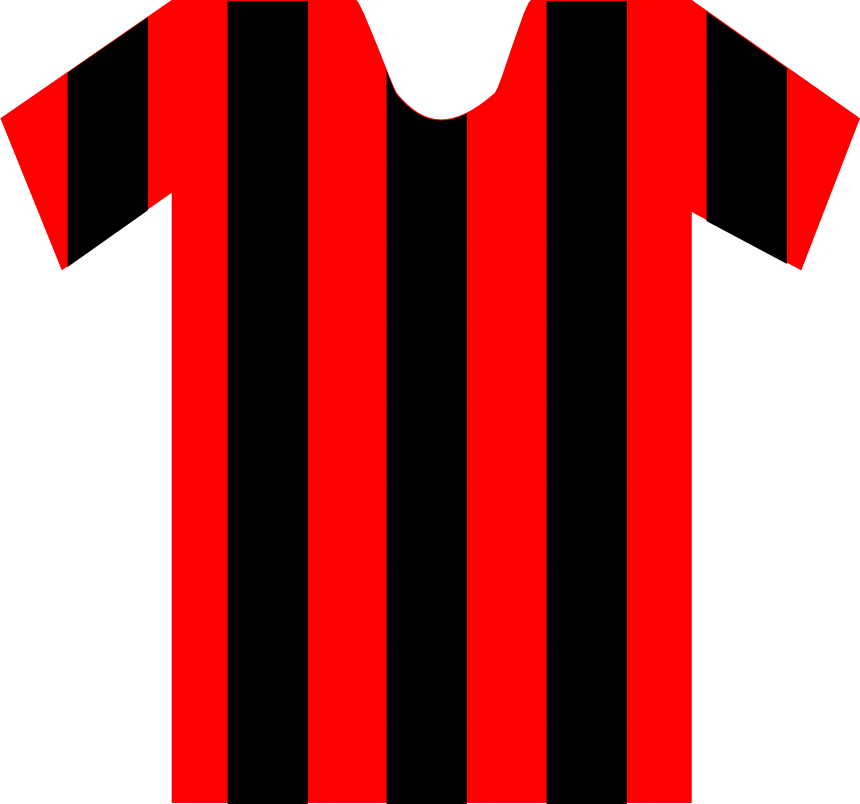
\includegraphics[width=.4\linewidth]{./images/rect2996.png}
        \captionof{figure}{Camiseta de 2 colores rayada. Las franjas de la camiseta son claramente distinguibles entre sí y el fondo.}
        \label{fig:camiseta-rayada}
    \end{minipage}
\end{figure}

Este es un desafío grande debido principalmente a dos problemas:
\begin{itemize}

\item Selección de colores: si la cancha tiene un color muy similar a la
  camiseta de un equipo, ¿cómo será posible distinguirlos? Se exploran
  distintas alternativas, como utilizar otra codificación de color.

\item Textura de los jugadores: esto representa un gran problema por varias
  razones. La primera es que la técnica de contornos activos está atada a la
  selección de una o varias características del objeto a seguir. Como la
  característica más distintiva es el color, la técnica se basá en ella. Pero
  para camisetas con más de un color, se vuelve absurda la idea de encontrar
  un color característico, dado que no existe.  Esta dificultad se ilustra en
  la imágenes de las figuras \ref{fig:barsa1} y \ref{fig:barsa2}. Por
  otro lado, dada la escasa cantidad de pixels que representan a un jugador,
  debido a nuestro enfoque de única cámara, cualquier tipo de análisis se torna
  complejo cuando sus características no están lo suficientemente definidas
  como para diferenciarlas (ya sea de otros jugadores o del fondo).

\end{itemize}

\begin{figure}[H]
    \centering
    \begin{minipage}{.5\textwidth}
        \centering
        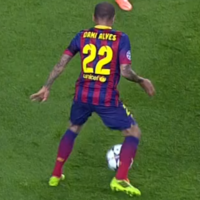
\includegraphics[width=.4\linewidth]{./images/resize_barcelona1.png}
        \captionof{figure}{Desde este punto de vista, se puede observar al menos 3 fuertes
        características (colores) en la camiseta del jugador, rojo, azul y amarillo.}
        \label{fig:barsa1}
    \end{minipage}%
    \begin{minipage}{.5\textwidth}
        \centering
        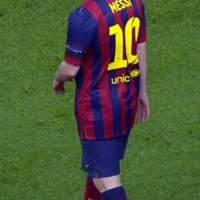
\includegraphics[width=.4\linewidth]{./images/resize_barcelona4.png}
        \captionof{figure}{Incluso con mayor resolución, las distintas características (como ser los colores azul, amarillo, y rojo) dificultan el seguimiento con contornos activos.}
        \label{fig:barsa2}
    \end{minipage}
\end{figure}

%TODO aca mepa que pueden ir varias imagenes.
% 1 de un tracking de de un jugador de remera blanca (podría ser PRE y POST, osea sin pintar y pintado)
% 1 de un tracking de un jugador de boca (again PRE y POST)
% 1 de la pelota? Para mostrar la cantidad infima de pixels?

